\documentclass[11pt,notitlepage]{article}
\usepackage{amsfonts, amsmath, amssymb, amsthm,fullpage,mdwlist}
\everymath{\displaystyle}
\newtheorem{thm}{Theorem}[section]
\title{$\mathbb{C}$alculus of Residues}
\author{Anish Tondwalkar}
\date{April Fools' 2011}
\begin{document}
\maketitle
Residue theory is a powerful tool to kill some integrals. Ideally, I'd prove everything I use, but we don't have the time for that on a Friday lecture, so I'll just do a few as examples. 
\section{Complex Integrals}
Since in the complex plane, we're now on a plane, not a line, there is more than one way to get from one point to another. Therefore, almost all the integrals you see during this lecture are going to be contour integrals. We define an integral along some path in $\mathbb{C}$ the same way we do in multivar for $\mathbb{R}^2$. One really trivial thing you should realize is that:
\begin{thm}[Cauchy's Integral Theorem]
$\oint_C f(z) dz = 0$ 
\end{thm}
\begin{flushright}
if $f$ is analytic (a.k.a.\! conservative) inside $C$ and continuous on $C$.
\end{flushright}
\section{Cauchy's Integral Formula}
\begin{thm}[Cauchy's Integral Formula]
$\oint_C \frac{f(z)}{z-z_0} dz = 2 \pi i f(z_0)$ 
\end{thm}
\begin{flushright}
if $f$ is analytic inside $C$.
\end{flushright}
\begin{proof}
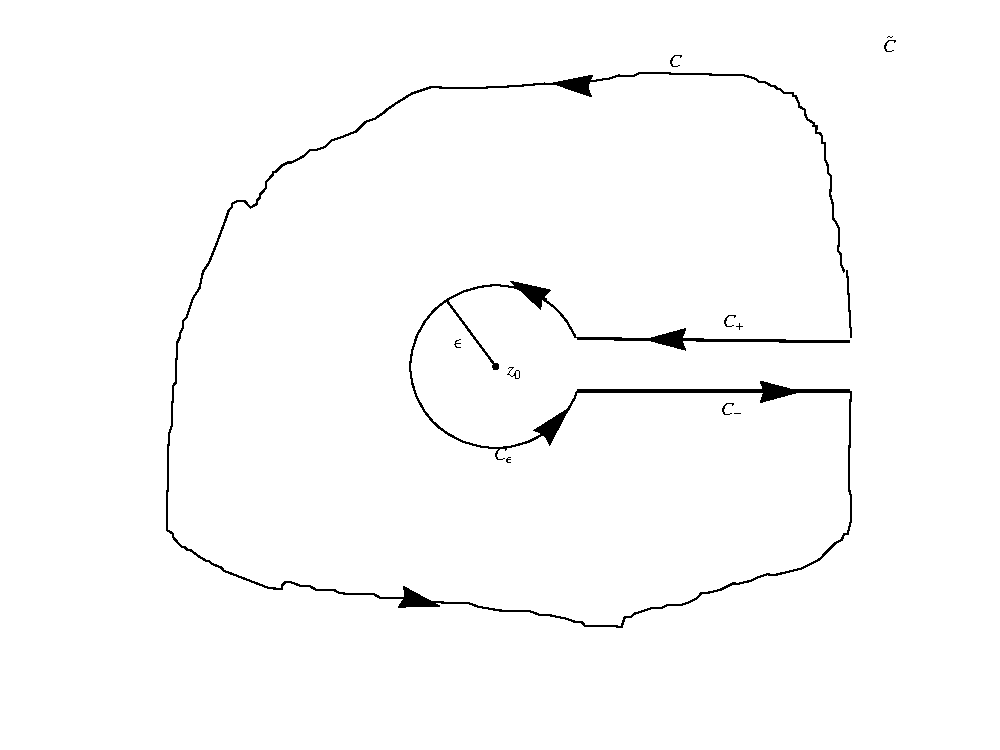
\includegraphics{ctwiddle}
$\twiddle C = C + \cancel{C_{+} + C_{-}}$

\end{proof}
\end{document}